\documentclass[fontset=ubuntu]{ctexart}

% \usepackage{ctex}
\usepackage{graphicx} % 图片
\usepackage{subfigure} %子图片
\usepackage{minted} % 代码
\usepackage{listings} % 代码
\usepackage{enumerate} % 有序列表
\usepackage{float} % 设置位置
\usepackage{hyperref} % 网页链接
\usepackage{fancyhdr} % 页眉页脚

\title{\Huge \textbf{实验报告四 \\ 调试与性能分析\&元编程\&大杂烩\&Pytorch}}
\author{\textit{潘奕霖}}
\date{https://github.com/PYL1024/system-develop-tools\\ \today}
\pagestyle{fancy}

\fancyhead{}
\fancyhead[R]{\textsl{\leftmark}}
\fancyfoot{}
\fancyfoot[L]{https://github.com/PYL1024/system-develop-tools}
\fancyfoot[R]{\thepage}
\setlength{\headheight}{14pt}
\addtolength{\topmargin}{-5pt}

\begin{document}

\maketitle
\newpage

\tableofcontents
\newpage

\section{调试与性能分析学习感悟}
性能分析给人的感觉就是东西很杂,有非常多的工具和非常多的用法,但是目前有很大一部分都还用不到。日志是日后工作中非常重要的一部分,而Linux提供的\mintinline{shell}| journalct|也确实是一个非常方便的工具,配合有关的参数和其他命令,能有效地管理日志。用pdb调试Python程序肯定没有Pycharm方便,但是pdb确实让调试工作变的很快捷。Python内部也提供了进行性能分析的工具,即cProfile,其能记录函数的调用时间,不过line profiler这样的工具则更为易用。像shellcheck这样的工具能检查shell脚本中的错误,Vim也有非常多的插件支持对不同编程语言的错误纠正和格式化,可以提高编程的效率。

\section{调试与性能分析知识点}
\subsection{查看日志}
\mintinline{shell}|journalctl|是journal control的简称。使用\mintinline{shell}| journalct|配合\mintinline{shell}|grep sudo|,查看超级用户的登录信息和执行的命令。
\begin{figure}[htb]
    \centering
    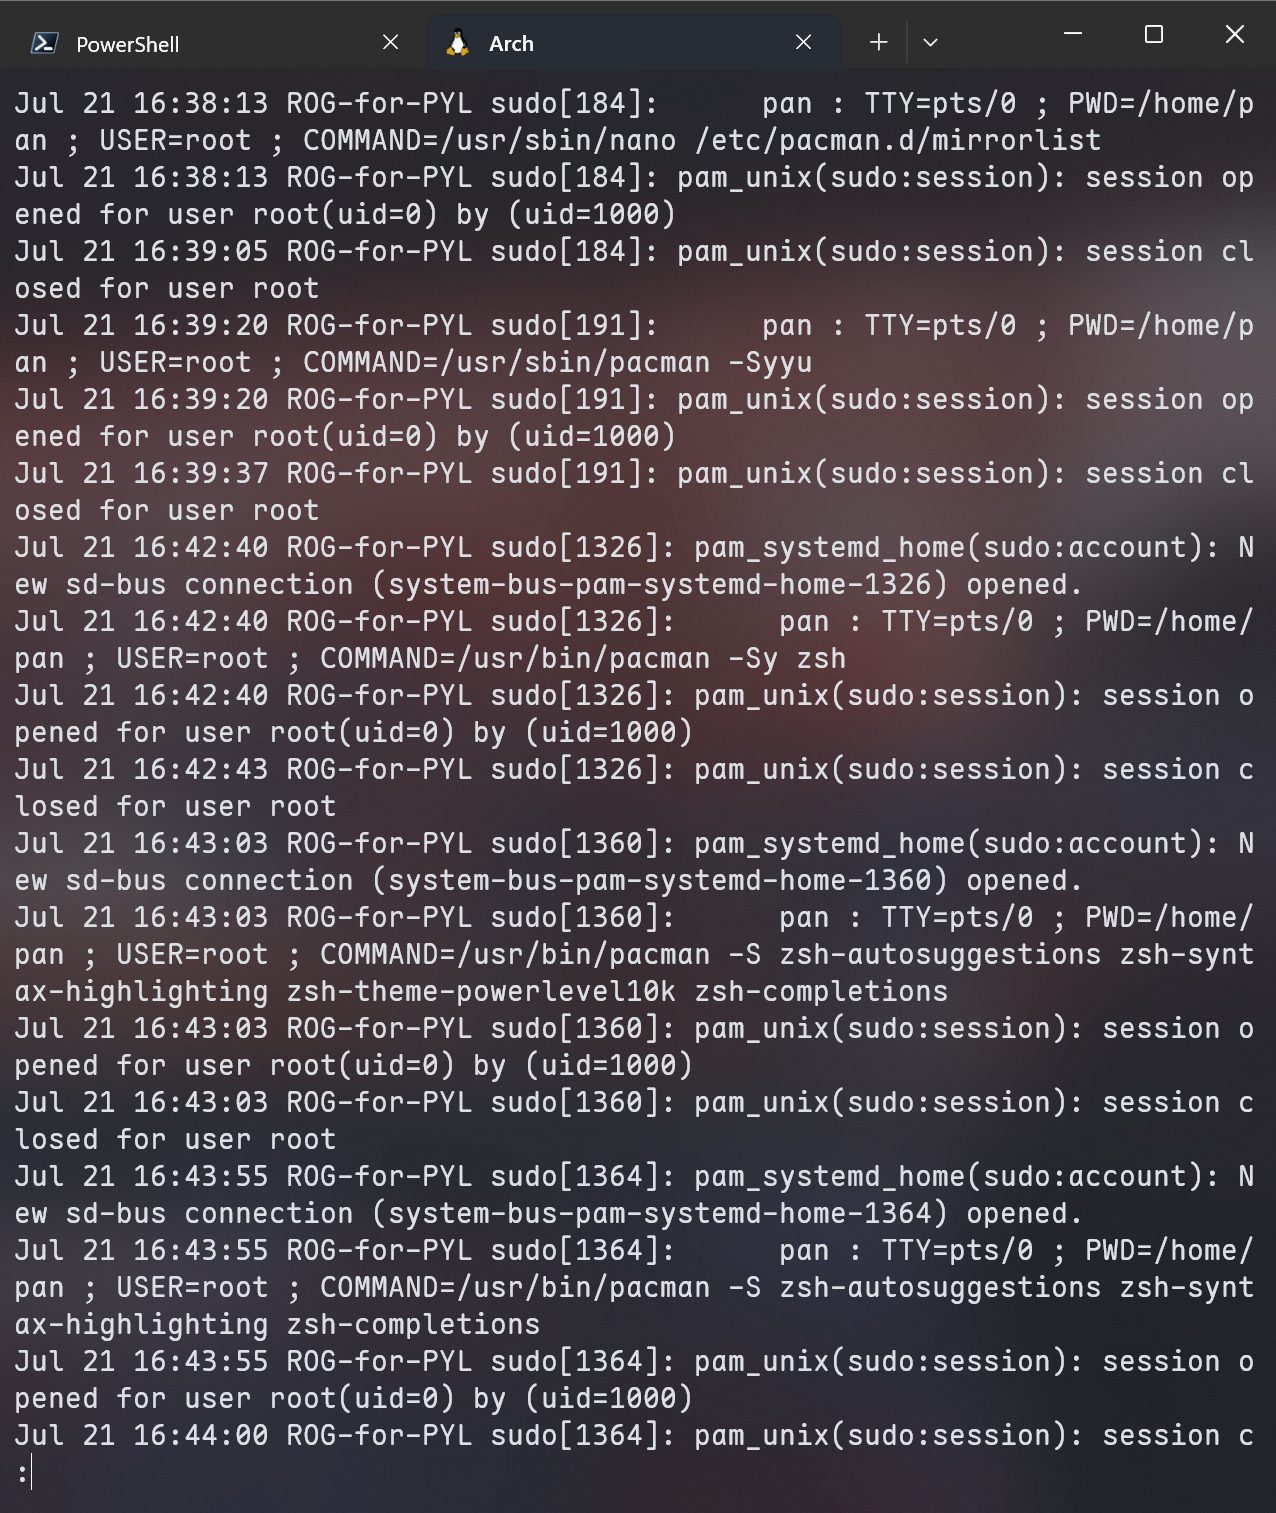
\includegraphics[width=0.5\linewidth]{journalctl_1.png}
    \caption{获取日志}
    \label{fig:journalctl_1}
\end{figure}

\subsection{写入日志并限定查看日志的时间范围}
使用\mintinline{shell}|logger|能写入日志,使用\mintinline{shell}|journalctl|命令的\verb|--since|或\verb|--until|参数可以限定查看日志的时间范围。可以指定具体的时间,也可以使用字符串,如"yesterday", "today", "tomorrow",还支持"ago"这样的表示方式,\verb|--since  "5m ago" |能将时间限定为五分钟以内。
\begin{figure}[htb]
    \centering
    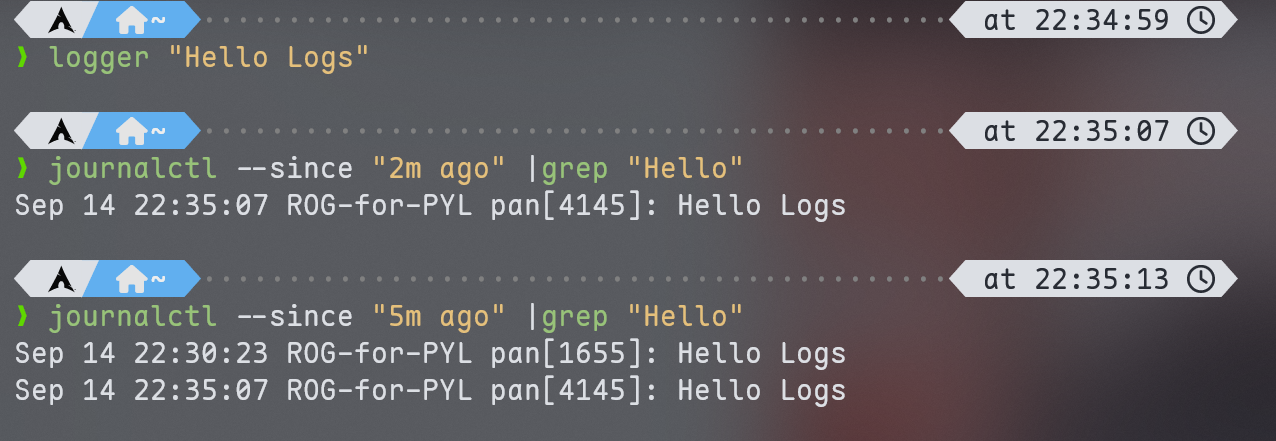
\includegraphics[width=0.75\linewidth]{journalctl_2.png}
    \caption{写入日志并查看}
    \label{fig:journalctl_2}
\end{figure}

\subsection{调试Python程序}
Python自带的调试工具是pdb。要使用pdb进行调试,有两种方式。不修改程序源代码的方式是用\verb|Python3 -m pdb filename.py|的方式运行程序;修改程序代码的方式则是导入包后,在要添加断点的地方加上\verb|pdb.set_trace()|,以在程序运行到此时暂停程序。在输入过\verb|n|或\verb|s|后,使用回车能再次执行命令,不用重复输入。
\begin{itemize}
    \item \verb|l| 查看当前代码段
    \item \verb|s| 进入函数
    \item \verb|n| 继续执行
    \item \verb|b| 设置断点,默认设置于当前行,但也可以指定行号
    \item \verb|p| 打印表达式的值
    \item \verb|r| 继续执行到当前函数返回
    \item \verb|q| 退出调试器
\end{itemize}

\subsection{对程序的运行进行计时}
通过使用Python的time模块,能对程序的运行进行计算。获取当前时间使用\mintinline{Python}|time.time()|,将运行后的时间减去运行前的时间就可以获取运行时间。
\begin{figure}[htb]
    \centering
    \subfigure[代码]{
    \label{fig:time_1}
     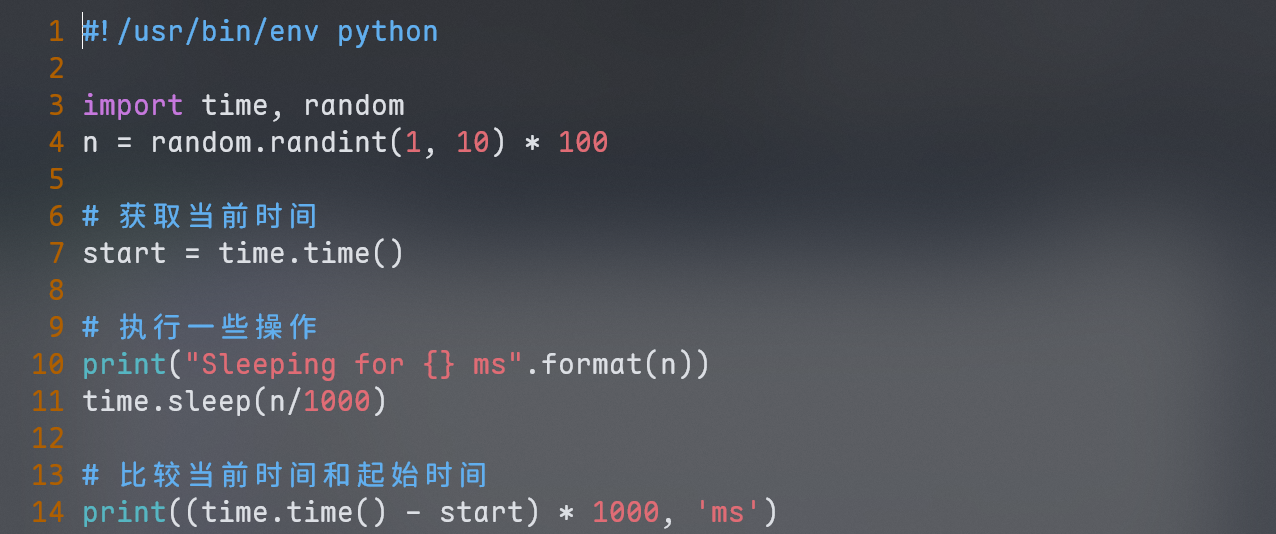
\includegraphics[width=0.45\linewidth]{time_1.png}
    }\subfigure[实现效果]{
     \label{fig:time_2}
    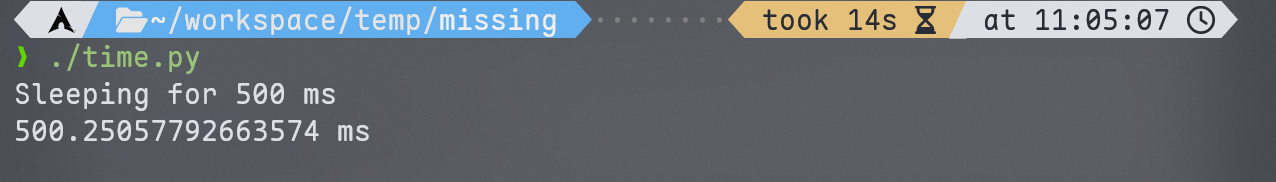
\includegraphics[width=0.45\linewidth]{time_2.png}
    }
    \caption{对程序运行进行计时}
    \label{time}
\end{figure}

\subsection{检查错误}
shellcheck可以检查shell脚本的错误,并给出修改建议。
\begin{figure}[htb]
    \centering
    \subfigure[有错误的脚本]{
    \label{fig:shellcheck_1}
    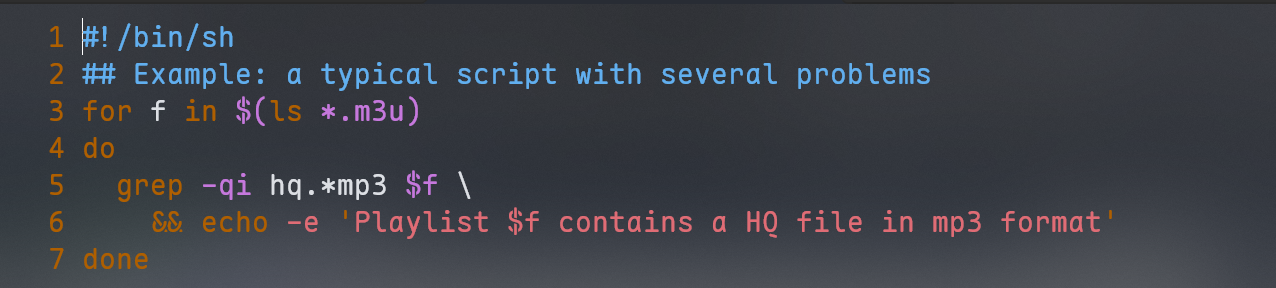
\includegraphics[width=0.45\linewidth]{shellcheck_1.png}
    }\subfigure[shellcheck检查出的错误]{
    \label{fig:shellcheck_2}
    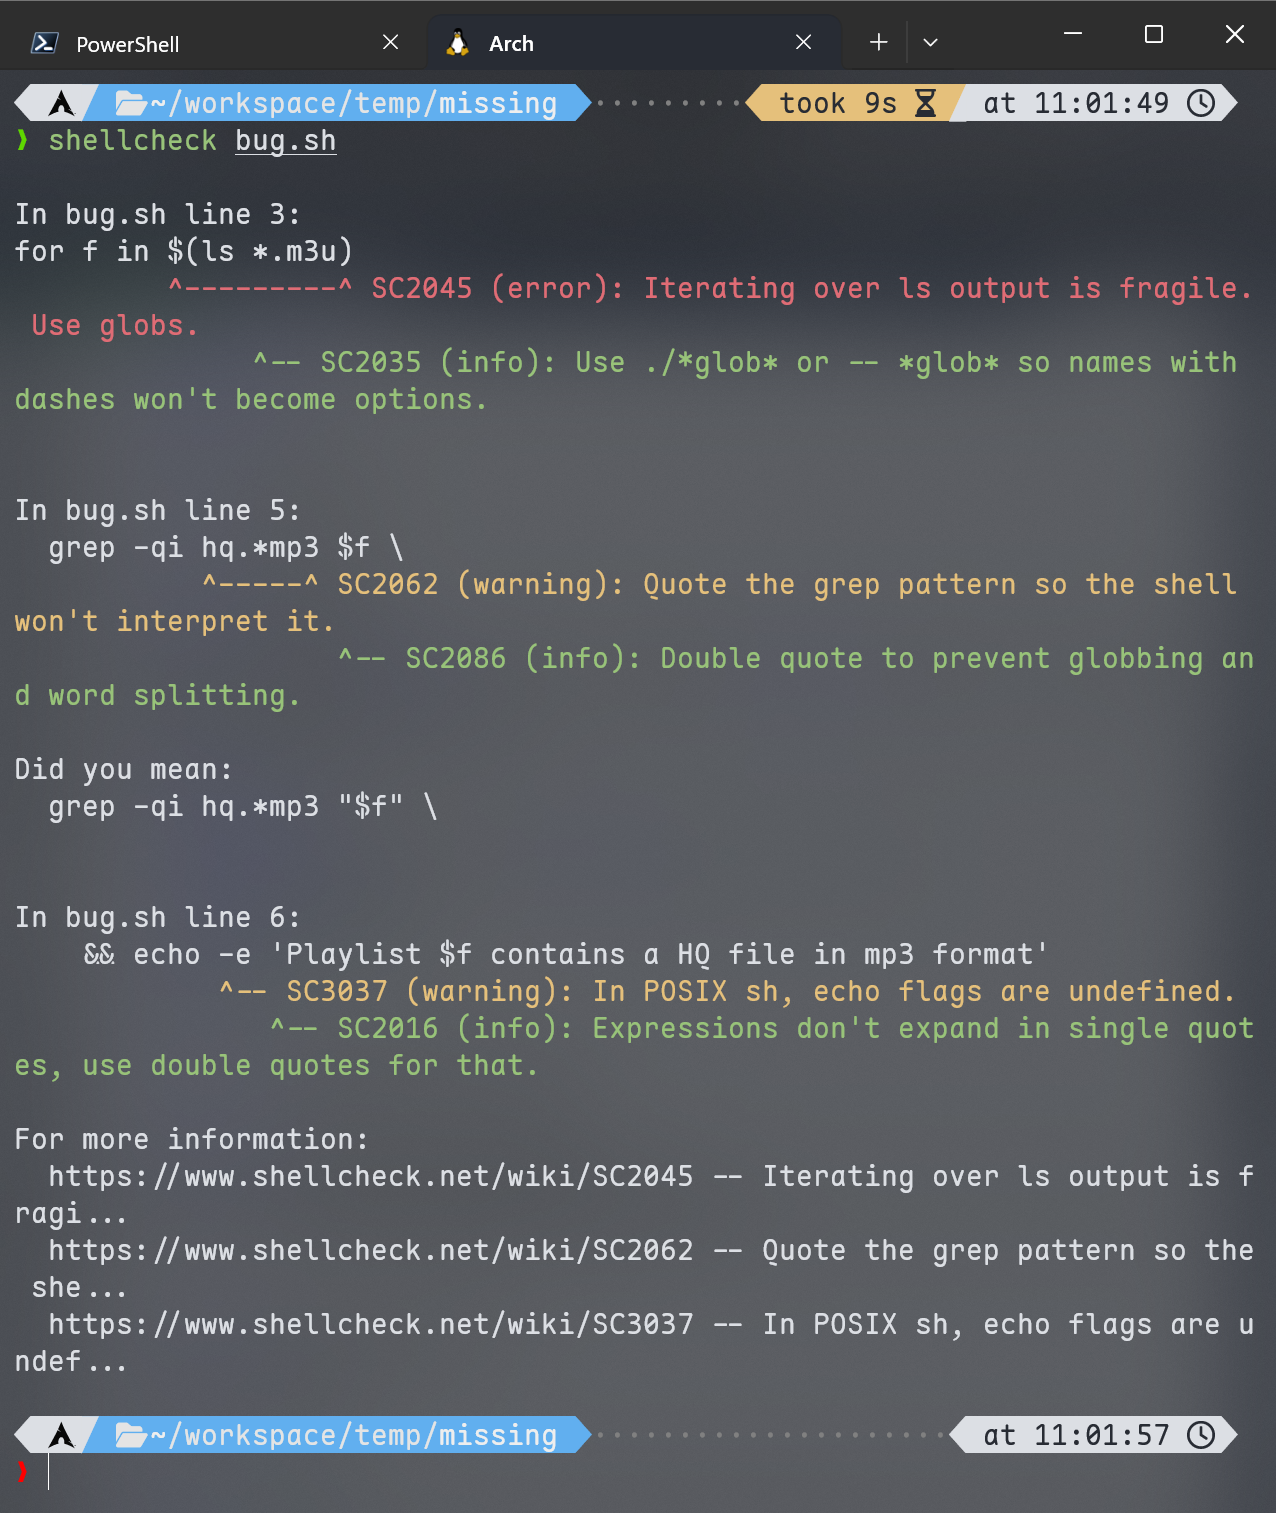
\includegraphics[width=0.45\linewidth]{shellcheck_2.png}
    }
    \caption{检查脚本错误}
   \label{shellcheck}
\end{figure}

像Pylint这样的工具可以检测Python代码中的错误,并实时进行显示。而autopep8配合Vim中的ale插件可以一键纠正代码格式,安装autopep8后在\verb|.vimrc|中添加\verb|let g:ale_fixers = { 'Python':['autopep8']}|,就可以在Vim中输入\verb|:ALEFix|来一键调整代码格式了。

\subsection{使用cProfile分析器查看函数调用时间}
但是由于是小程序,函数的调用时间都非常的短。
\begin{figure}[htb]
    \centering
    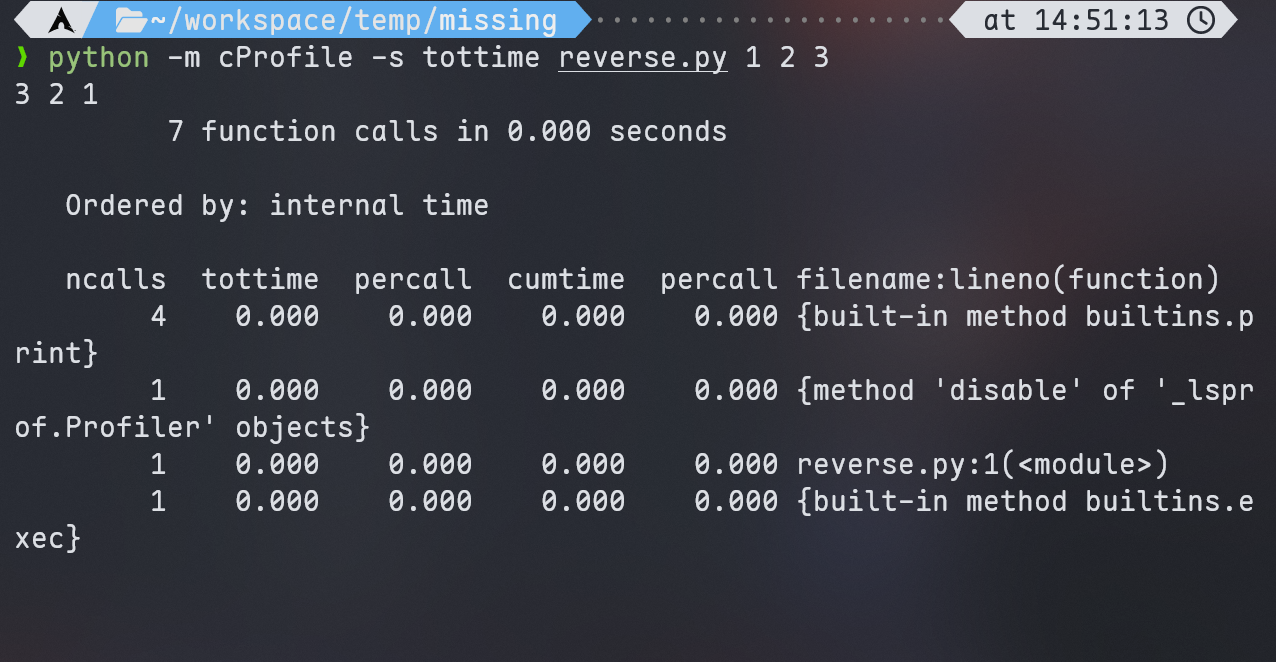
\includegraphics[width=0.5\linewidth]{cProfile_1.png}
    \caption{查看函数调用时间}
    \label{fig:cProfile_1}
\end{figure}

\subsection{使用htop查看监控}
在安装完htop后,只要输入\mintinline{shell}|htop|就能启动htop,对系统进行监控。
\begin{figure}[htb]
    \centering
    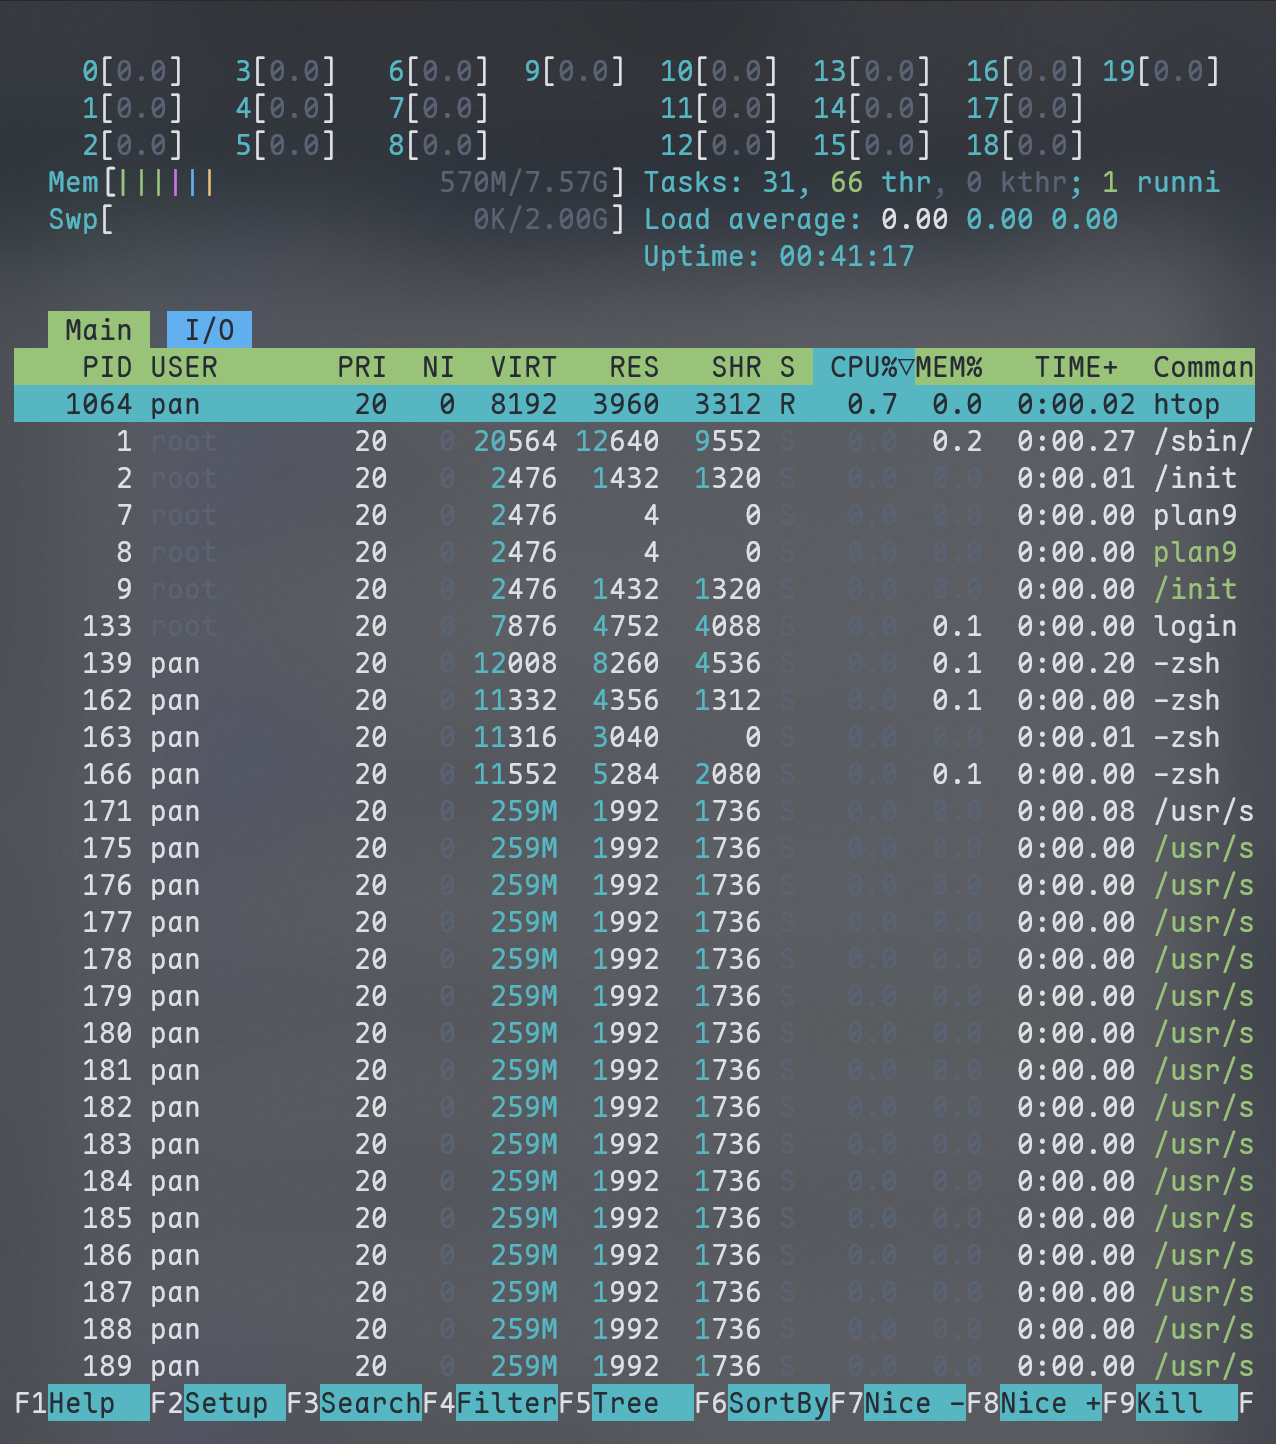
\includegraphics[width=0.5\linewidth]{htop_1.png}
    \caption{查看监控}
    \label{fig:htop_1}
\end{figure}

\section{元编程学习感悟}
元编程是一个挺抽象的概念,包括了构建、版本控制和持续集成。我感觉只能非常浅地了解一下。

\section{元编程知识点}
\subsection{构建项目}
使用\mintinline{shell}|make|来构建项目,其会参考Makefile文件。该文件内包含了构建项目所需要的各种指令。文件的形式为:
\begin{listing}[htb]
    \begin{verbatim}
    A: B C
        <command>
    D%: E%
        <command>
    \end{verbatim}
\end{listing}

使用右侧的文件构建左侧的文件,缩进部分为构建时所需要的命令。\%会匹配冒号左右两侧相同的字符串。

\subsection{版本控制}
使用版本号对版本进行管理。相对比较常用的语义版本号格式为:主版本号.次版本号.补丁号。使用规则是如果新版本没有改变API,将补丁号递增;添加API且向后兼容,将次版本号递增;修改API但不向后兼容,将主版本号递增。详细信息可以查看这个\href{https://semver.org/}{网站}。

\subsection{持续集成}
持续集成给人一种自动化的感觉。如利用Github Action的shellcheck在提交新的代码后对其进行检查。进入仓库的action页面,点击Simple workflow下的Configuration按钮,进入.yml文件的编辑页面。在这个页面的右侧可以搜索相关的插件,搜索shellcheck并将安装语句复制到自己的.yml文件中,点击右上角提交更改,就能对提交的代码进行shellcheck了。
\begin{figure}[htb]
    \centering
    \subfigure[进入编辑页面]{
    \label{fig:action_1}
    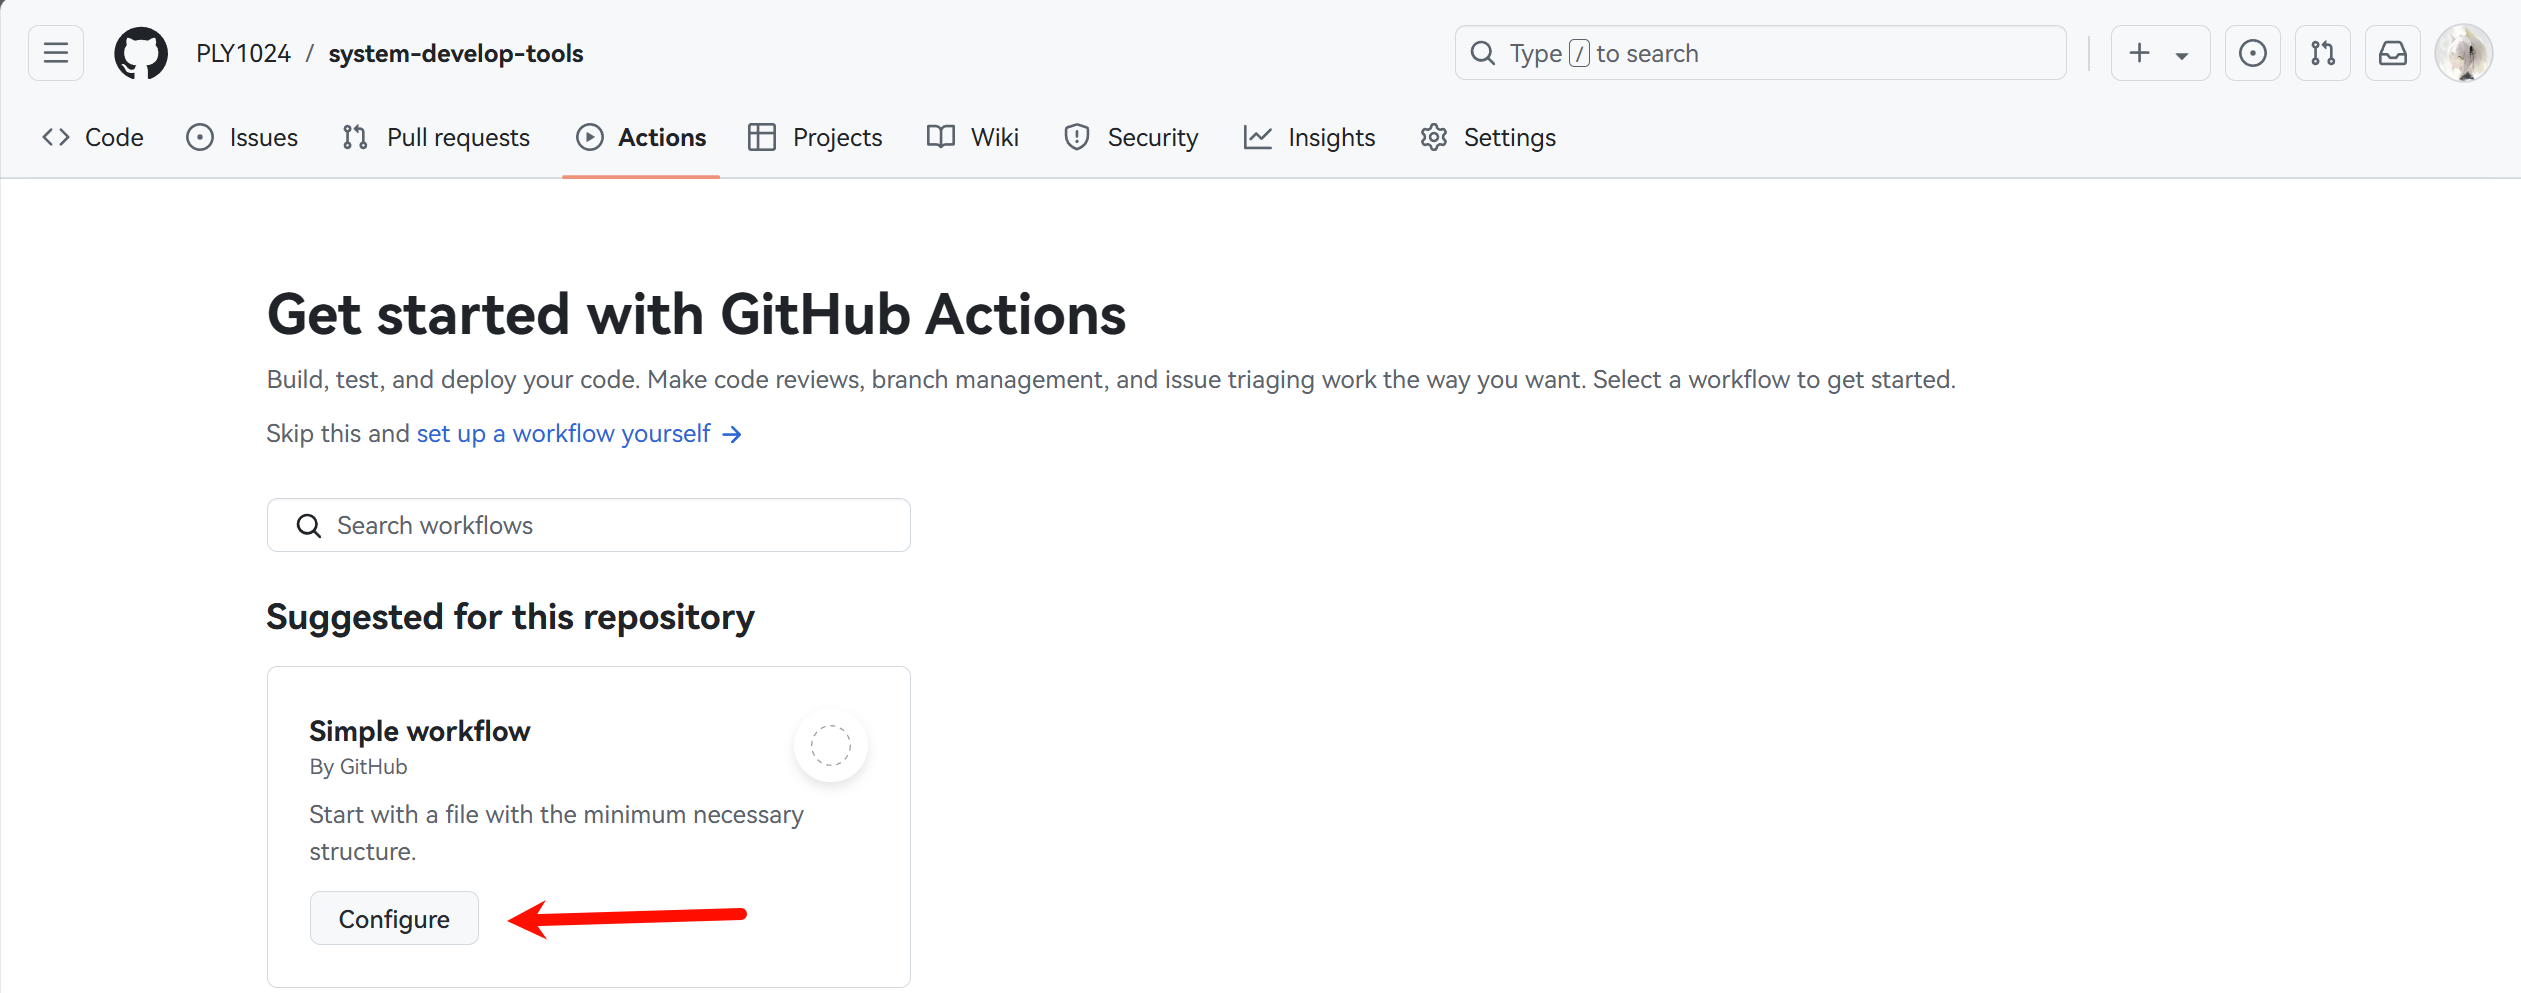
\includegraphics[width=0.45\linewidth]{action_1.png}
    }\subfigure[安装shellcheck]{
    \label{fig:action_2}
    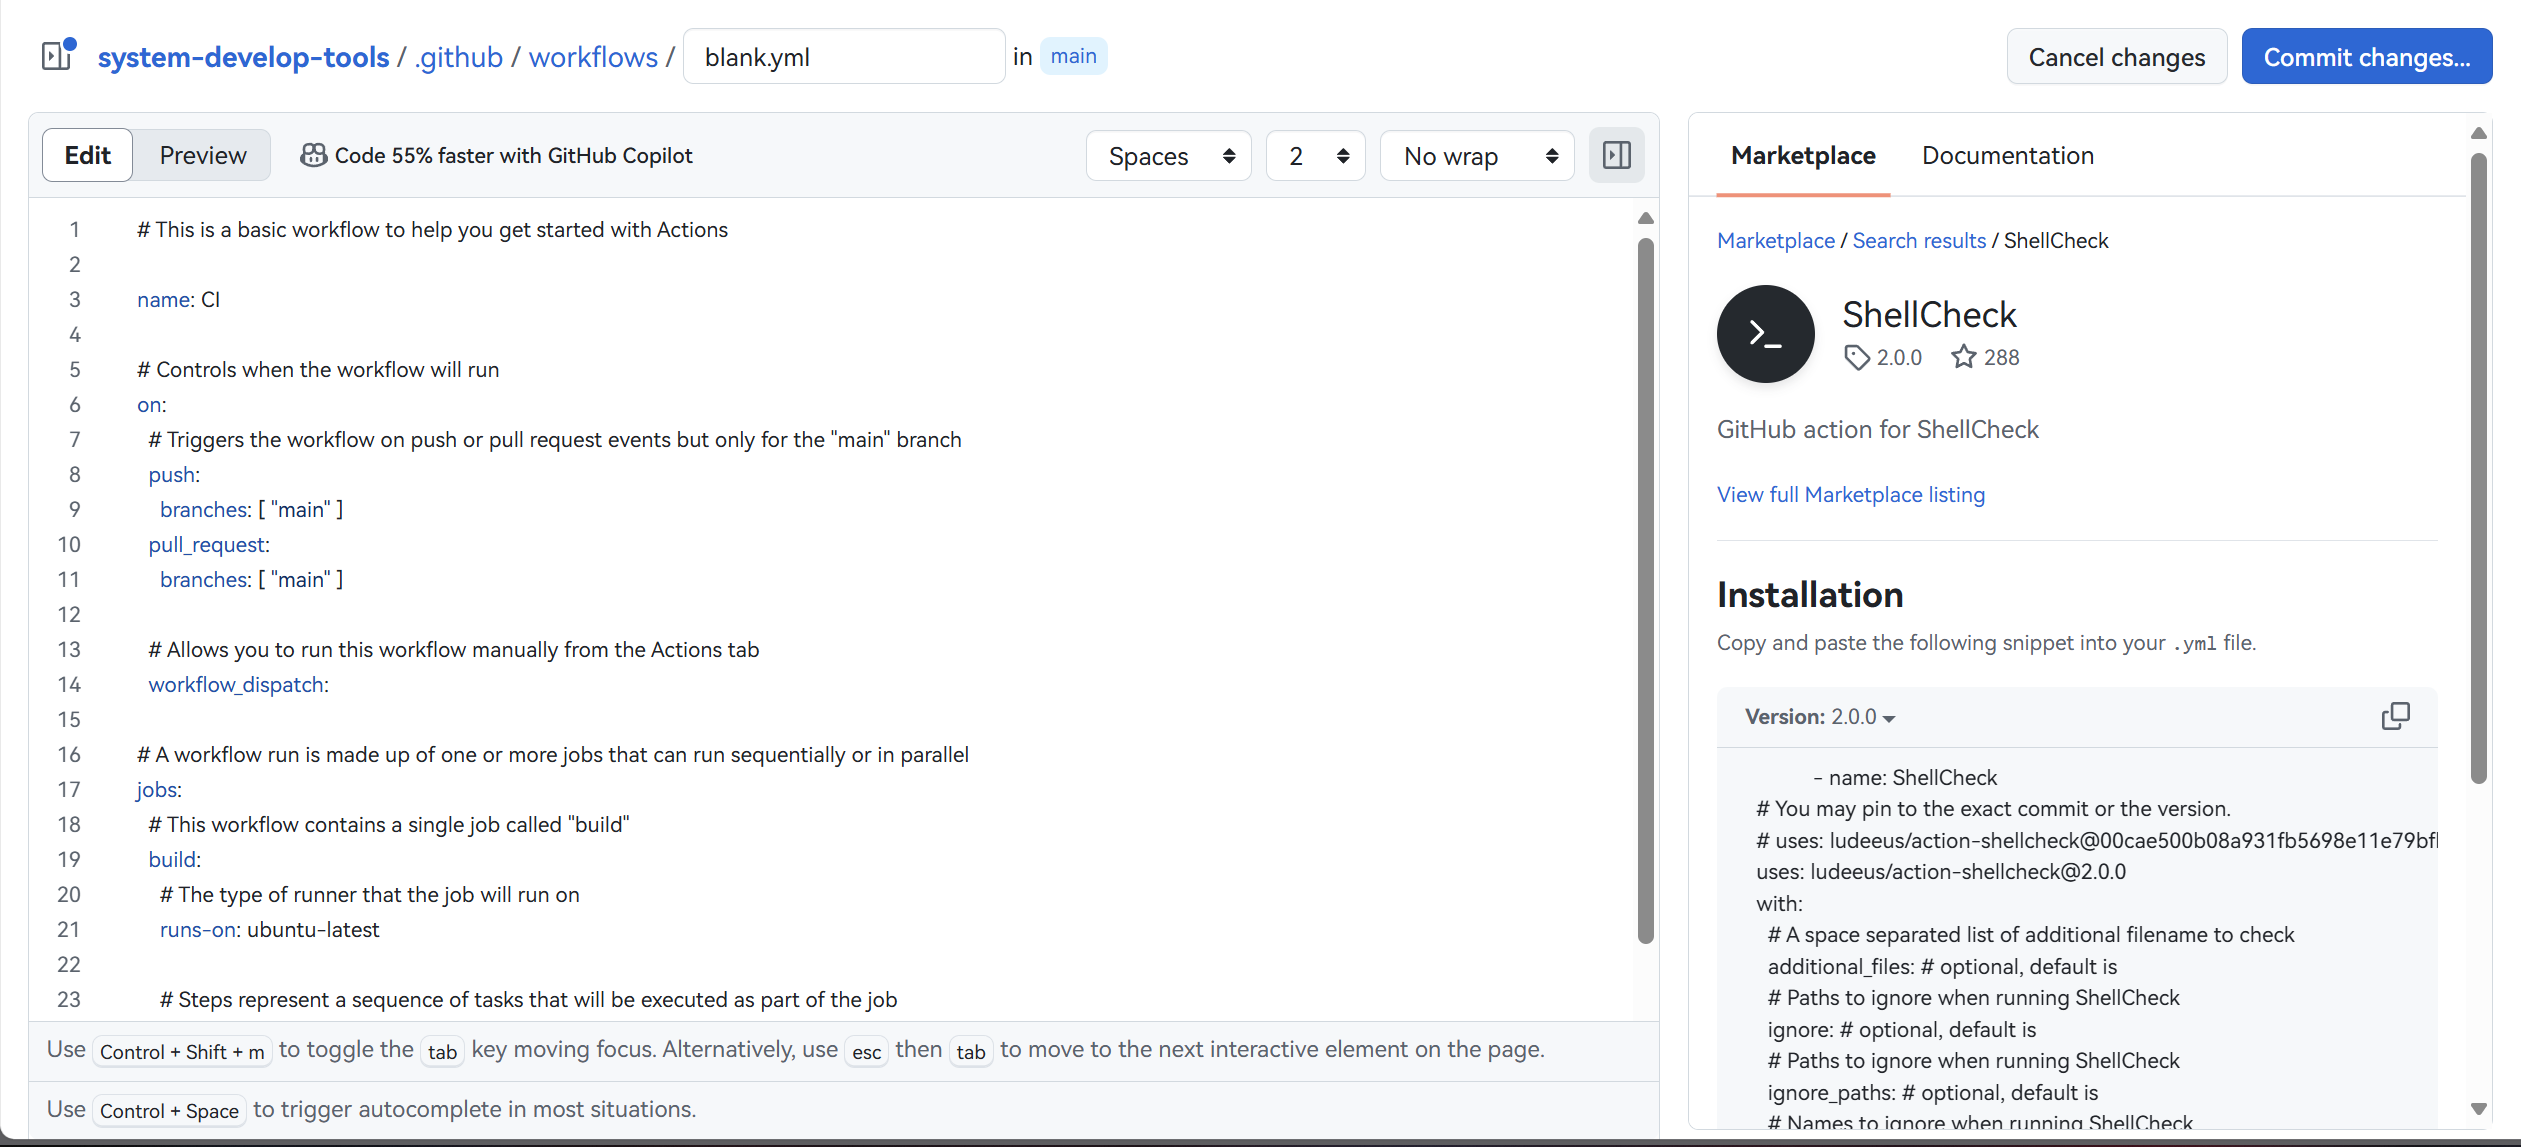
\includegraphics[width=0.45\linewidth]{action_2.png}
    }
    \caption{使用Github Action}
    \label{action}
\end{figure}

\section{大杂烩学习感悟}
大杂烩的内容确实杂,杂到我觉得有一点不太用的到。除了Markdown和与API有关的IFTTT外,别的知识点都离我们太远了。

\section{大杂烩知识点}
\subsection{IFTTT}
IFTTT代表if this then that,其能在多个事件之间建立联系。其网站上提供了许多有趣有用的小程序,如当国际空间站经过你家时告诉你,定时发送天气预报等。还能实现许多跨平台的功能,比如将苹果手机的通讯录保存到谷歌云盘,或者对物品的价格进行监控。

\subsection{Markdown语法}
\begin{itemize}
    \item \# 设置标题,\#越多,标题越小
    \item \verb|*| 设置斜体 
    \item \verb|**| 设置粗体
    \item \verb|-| 表示无序的列表的元素
    \item 数字序号加\verb|.| 表示有序列表元素
    \item \verb|`| 包围的内容会以代码的形式展示,使用\verb|```|包围文字以显示代码块
    \item \verb|>| 设置引用的内容
\end{itemize}

\section{PyTorch学习感悟}
安装是学习PyTorch的第一步,也是非常劝退的一步。其安装流程不仅长,而且也有不少的注意点。

在按步骤操作完教程后,我只能说写出PyTorch的人简直是天才,能用相对简单的方式把对神经网络的操作写成函数给调用者使用,还能达到如此神奇的效果。这些函数背后的实现方式简直无法让我想象,通过几个参数就能获得模型的各个参数,而且还能通过不同的方式对权重进行修改,还能让模型依据要求进行训练,实在是神奇。

要学好PyTorch,掌握其运用方式肯定是不够的,需要理解其背后的实现方式,才能真正用好PyTorch,否则这些函数和调优方法还是像黑箱一样,知道输出结果而不知道其内部结构。

\section{PyTorch知识点}
\subsection{安装CUDA® Toolkit}
安装CUDA® Toolkit是安装PyTorch第一步。先检查自己电脑的显卡驱动支持到哪个版本的CUDA® ,在命令行中输入\mintinline{shell}|nvidia-smi|,会列出有关显卡的信息,也会显示显卡驱动支持的最高版本CUDA® 。
\begin{figure}[htb]
    \centering
    \includegraphics[width=0.5\linewidth]{Cuda_1.png}
    \caption{查看显卡驱动支持的CUDA®版本}
    \label{fig:Cuda_1}
\end{figure}

我的显卡驱动支持12.5版本的CUDA®,前往CUDA®的\href{https://developer.nvidia.com/cuda-toolkit-archive}{下载网站}选择对应的版本进行下载。在下载完安装包后运行进行安装即可。安装时可以选择自定义安装,避免CUDA®被安装到C盘,占据宝贵的空间。

安装完成后,在命令行输入\mintinline{shell}|nvcc -V|,若能正确输出信息,则安装成功。
\begin{figure}[htb]
    \centering
    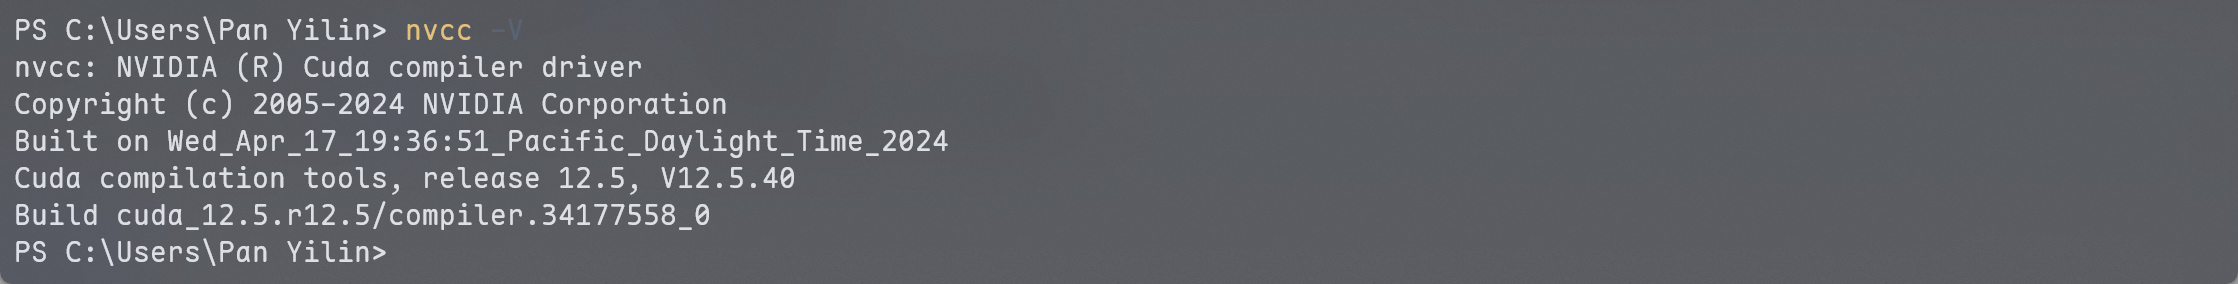
\includegraphics[width=0.75\linewidth]{Cuda_2.png}
    \caption{输出的信息}
    \label{fig:Cuda_2}
\end{figure}

\subsection{安装Anaconda®}
接下来安装Anaconda®。Anaconda® 是一个包管理器、一个环境管理器、一个 Python/R 数据科学发行版以及超过 7,500 个开源包的集合,在PyTorch的使用中非常重要。

前往Anaconda®的\href{https://www.anaconda.com/download/success}{下载网站}进行下载,这里没什么要注意的。在下载完成后运行安装程序,同样可以把安装位置修改为C盘以外的地方。

在安装完成后,打开Anaconda Prompt,就可以在命令行中使用Anaconda®,或者使用图像化的Anaconda Navigator。不过在安装完成后要记得换源。
\begin{figure}[htb]
    \centering
    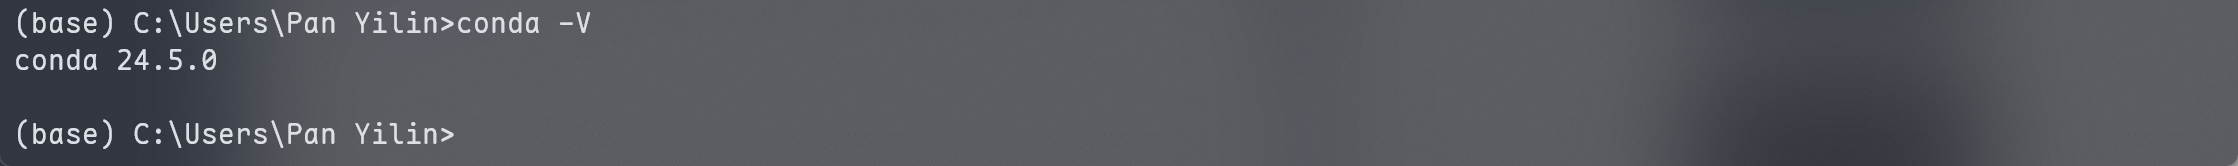
\includegraphics[width=0.75\linewidth]{conda_1.png}
    \caption{Anaconda Prompt}
    \label{fig:conda_1}
\end{figure}

\subsection{安装PyTorch}
接下来就可以安装PyTorch了。首先在Anaconda Prompt中为PyTorch创建一个虚拟环境,用\verb|conda create -n pytorch version=3.11|创建一个Python版本为3.11的虚拟环境,因为Pytorch目前还不支持Python3.12。可以使用\verb|conda env list|列出当前所有的虚拟环境。
\begin{figure}[htb]
    \centering
    \subfigure[列出虚拟环境]{
    \label{fig:conda_2}
    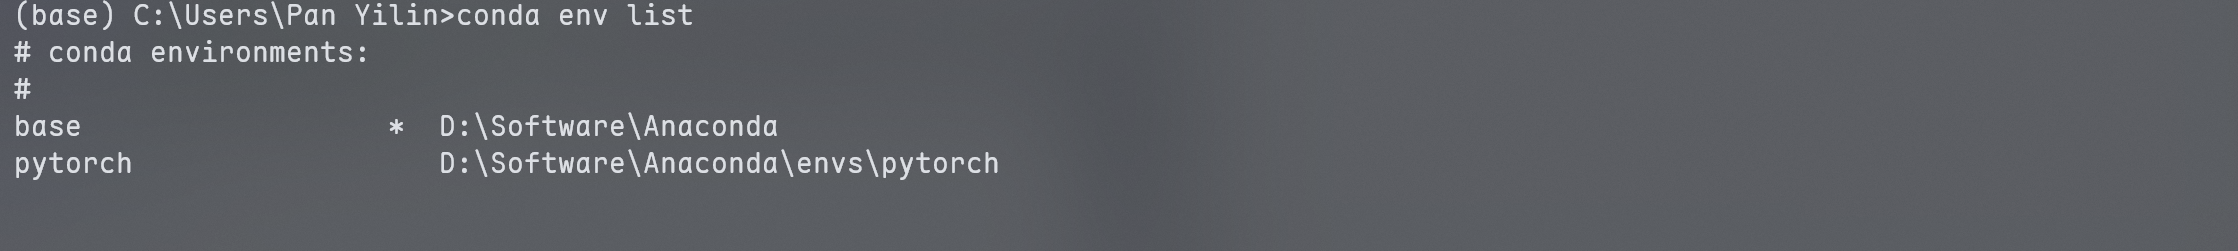
\includegraphics[width=0.45\linewidth]{conda_2.png}
    }\subfigure[激活虚拟环境]{
    \label{fig:conda_3}
    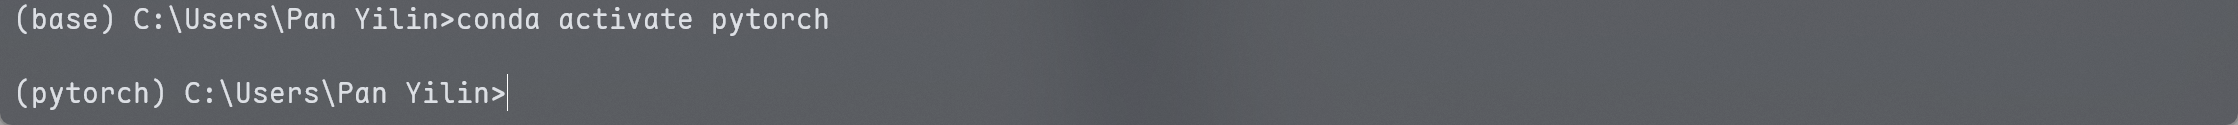
\includegraphics[width=0.45\linewidth]{conda_3.png}
    }
    \caption{虚拟环境}
    \label{conda}
\end{figure}

使用\verb|conda activate pytorch|激活刚刚创建的虚拟环境,此时路径前的\verb|base|会变为\verb|pytorch|。

前往PyTorch的\href{https://pytorch.org/get-started/locally/}{下载网站},按照需求进行选择,复制安装命令至虚拟环境中运行,PyTorch就会开始下载。
\begin{figure}[htb]
    \centering
    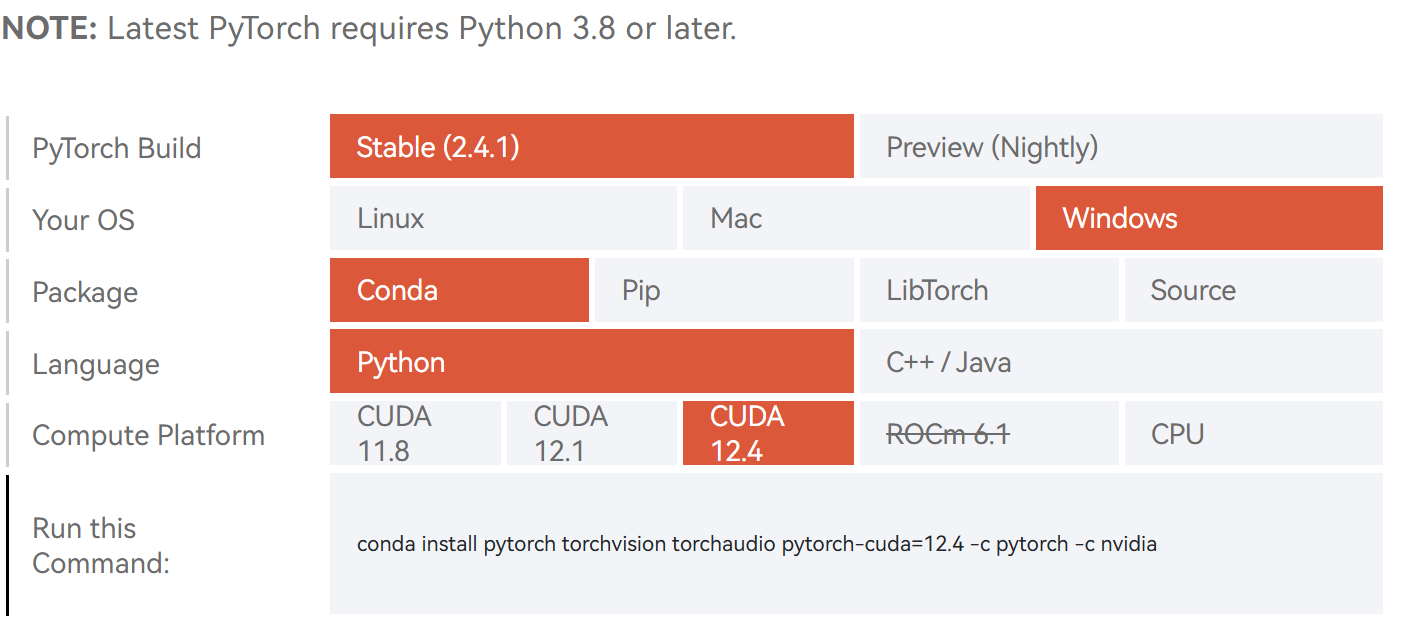
\includegraphics[width=0.5\linewidth]{conda_4.png}
    \caption{下载选项}
    \label{fig:conda_4}
\end{figure}

要检验安装是否成功,在虚拟环境中输入\verb|Python|进入Python交互式环境,输入以下代码:
\begin{listing}[htb]
    \begin{minted}{Python}
    import torch
    x = torch.rand(5, 3)
    print(x)
    \end{minted}
\end{listing}

注意包名是torch,如果能成功输出类似以下的内容,那么PyTorch就安装成功了。如果输入\verb|torch.cuda.is_available()|,若返回\mintinline{Python}|true|,则显卡也能被调用,大功告成。
\begin{figure}[htb]
    \centering
    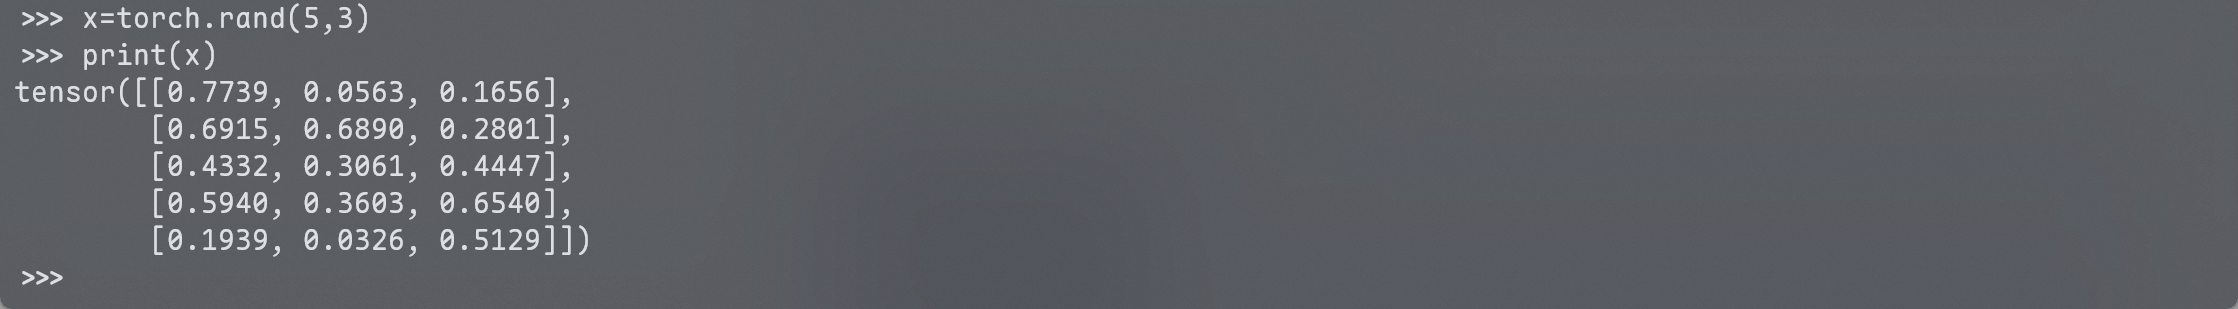
\includegraphics[width=0.75\linewidth]{conda_5.png}
    \caption{安装成功}
    \label{fig:conda_5}
\end{figure}

\subsection{张量的初始化}
Tensor,中文翻译为张量,实际上为一个多维数组。有多种方式可以对其初始化。张量默认存放在CPU上,使用\mintinline{Python}|tensor.device|获取张量储存的位置。使用\mintinline{Python}|tensor.to('cuda')|可以将其移动到GPU。CPU上的张量和NumPy数组可以共享它们的底层内存位置,改变一个就会改变另一个。比如以一个NumPy数组产生张量后,对张量的修改操作也会反映在NumPy数组上。同样的,一个张量可以转为NumPy数组,而对这个数组进行修改也就能对张量进行修改。

由数据初始化,即Python内的列表,可以指定多维列表,也不用考虑数据类型;或由NumPy数组初始化:
\begin{listing}[htb]
    \begin{minted}{Python}
    data = [[1, 2], [3, 4]]
    x_data = torch.tensor(data)
    \end{minted}    
\end{listing}

\begin{listing}[htb]
    \begin{minted}{Python}
    np_array = np.array(data)
    x_np = torch.from_numpy(np_array)
    \end{minted}    
\end{listing}

由另一个张量初始化,保留参数张量的属性(形状,数据类型),除非显示覆盖:
\begin{listing}[htb]
 \begin{minted}{Python}
    x_ones = torch.ones_like(x_data)
    print(f"Ones Tensor: \n {x_ones} \n")

    x_rand = torch.rand_like(x_data, dtype=torch.float)
    print(f"Random Tensor: \n {x_rand} \n")
 \end{minted}    
\end{listing}

\subsection{张量操作}
张量支持类似矩阵乘法,拼接,元素对应乘法、索引切片等操作。
\begin{itemize}
    \item 切片 \mintinline{Python}|tensor[:, 1]|
    \item 拼接 \mintinline{Python}|torch.cat([tensor, tensor,], dim=1)|
    \item 元素乘积 \mintinline{Python}|tensor.mul(tensor)|
    \item 矩阵乘积 \mintinline{Python}|tensor.matmul(tensor.T)|
\end{itemize}

\mintinline{Python}|tensor.T|即将tensor转置。

\subsection{Autograd}
Autograd能帮助神经网络自动进行训练。训练一个神经网络分为两个步骤:前向传播与反向传播。向前传播即神经网络做出猜测,而反向传播时神经网络会调整其参数以减小误差。

对一个模型,先进行向前传播做出预测,再通过预测和相对应的标签计算出预测的误差,再使用\mintinline{Python}|backward|函数反向传播,这时Autograd会计算并储存模型参数的梯度。

要对参数进行调整,需要使用优化器。优化器使用如下的语句加载模型参数并设定学习率和动量。使用\mintinline{Python}|optim.step()|启动优化器,其就会根据储存的梯度调整参数。

\subsection{一个神经网络的构建过程}
一个神经网络的构建包括四步,定义神经网络,输入与反向传播,计算损失,更新权重。

定义过程包括了初始化与编写\mintinline{Python}|forward|函数,而\mintinline{Python}|backward|函数由autograd帮我们定义。

运行教程中的代码,得到的输出是:
\begin{figure}
    \centering
    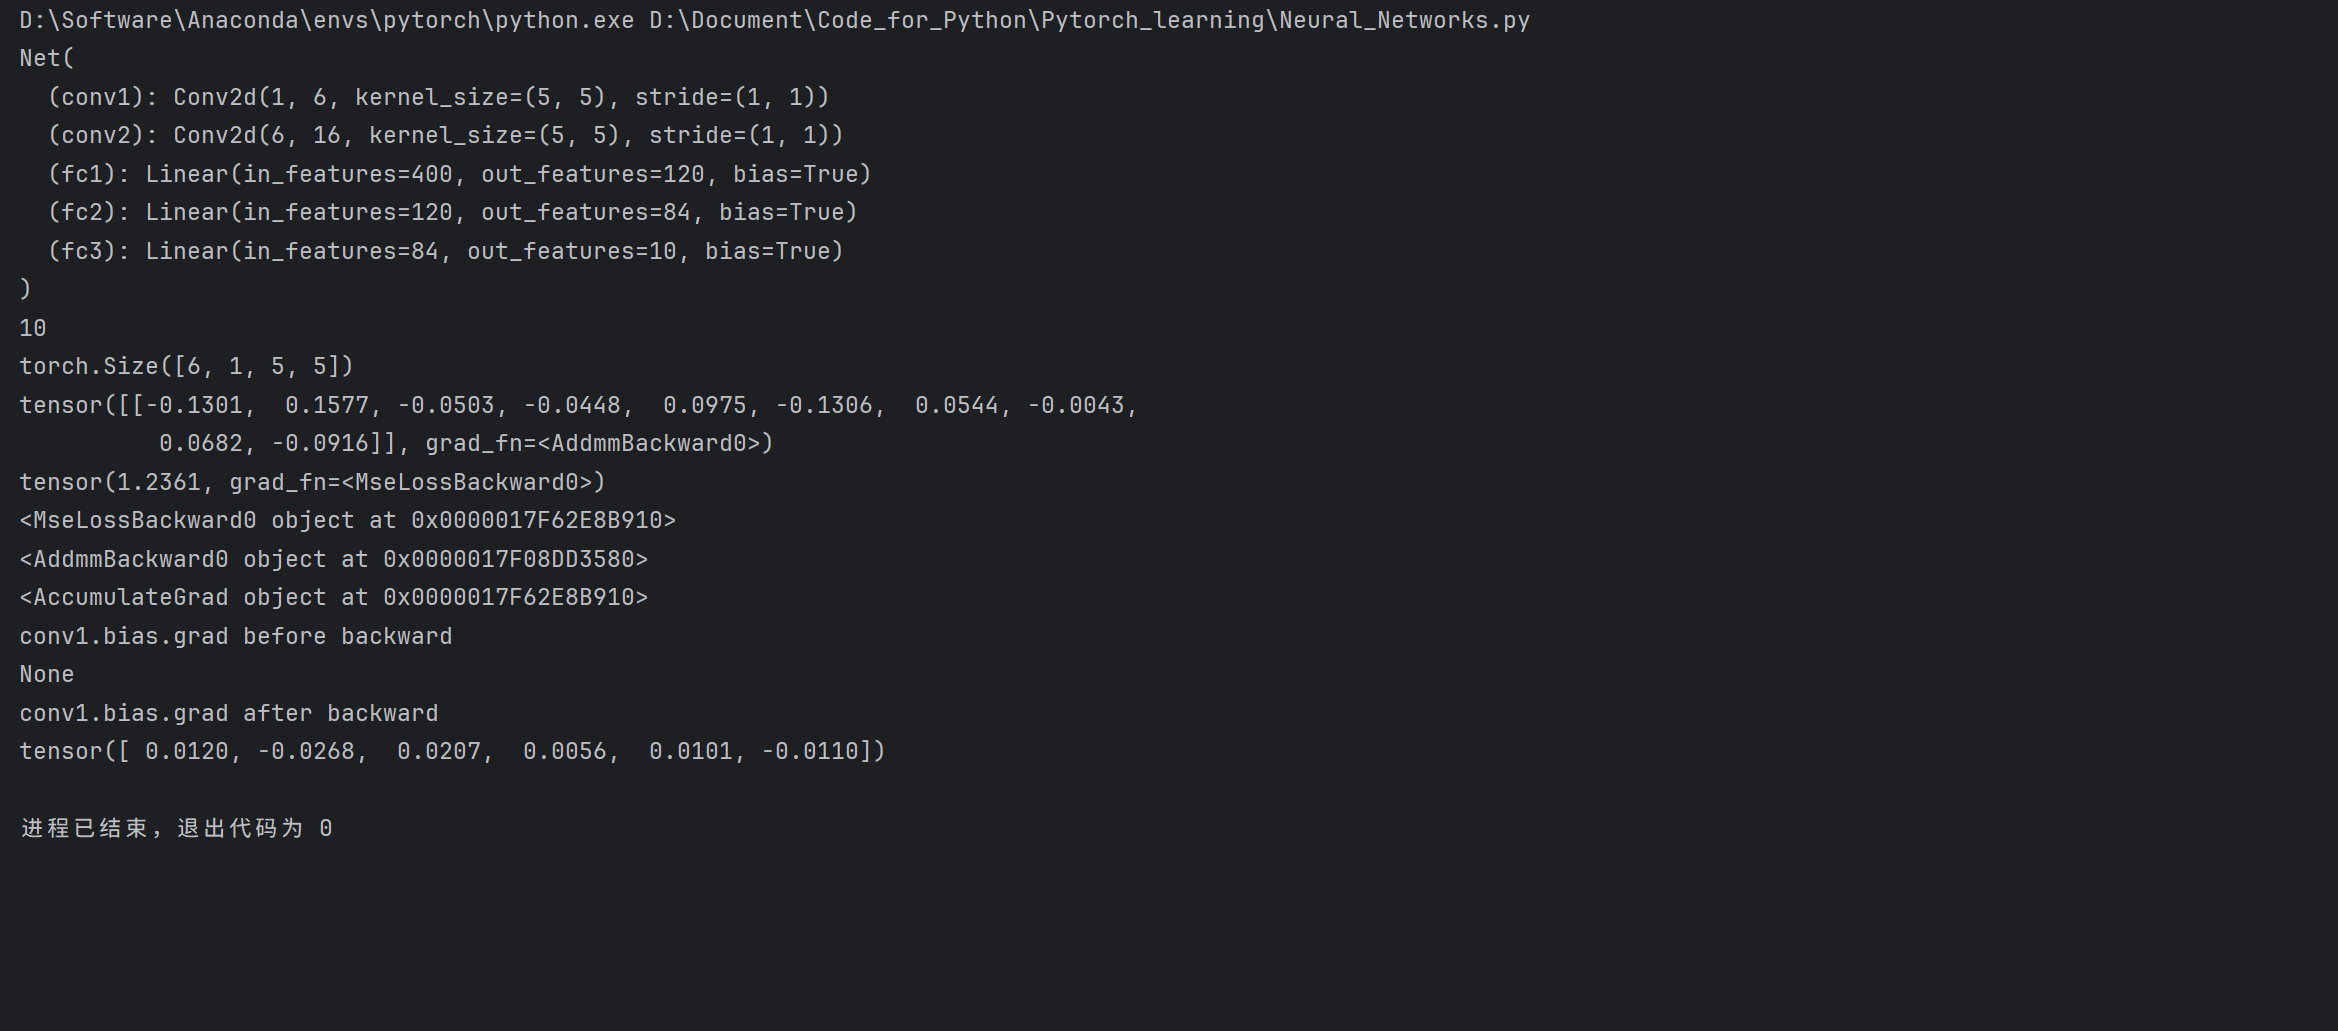
\includegraphics[width=0.75\linewidth]{PyTorch_1.png}
    \caption{输出结果}
    \label{fig:PyTorch_1}
\end{figure}

\subsection{训练一个图像识别模型}
根据教程代码,进行训练:
\begin{figure}[htb]
    \centering
    \subfigure[训练过程]{
    \label{fig:PyTorch_2}
    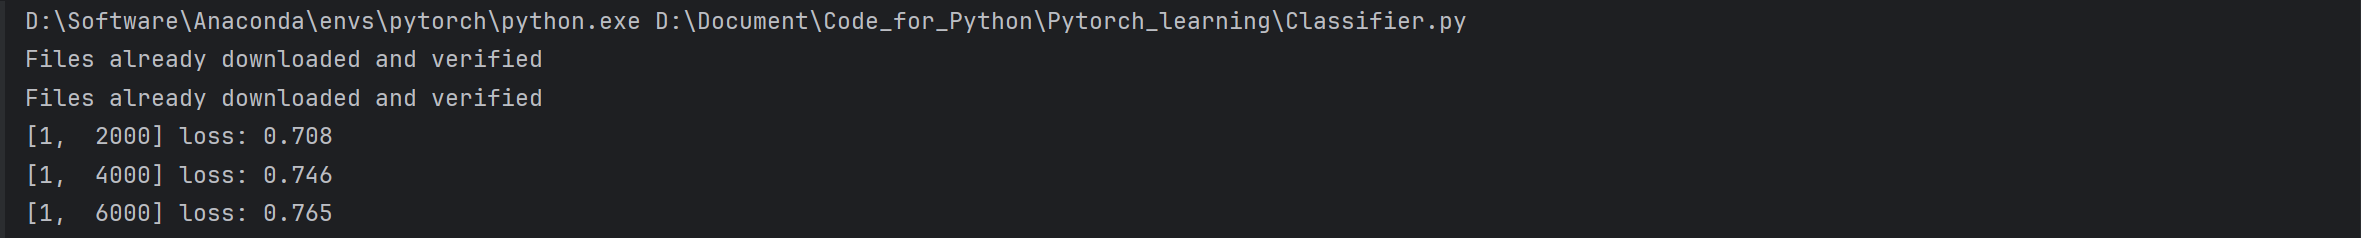
\includegraphics[width=0.45\linewidth]{PyTorch_2.png}
    }\subfigure[识别结果]{
    \label{fig:PyTorch_3}
    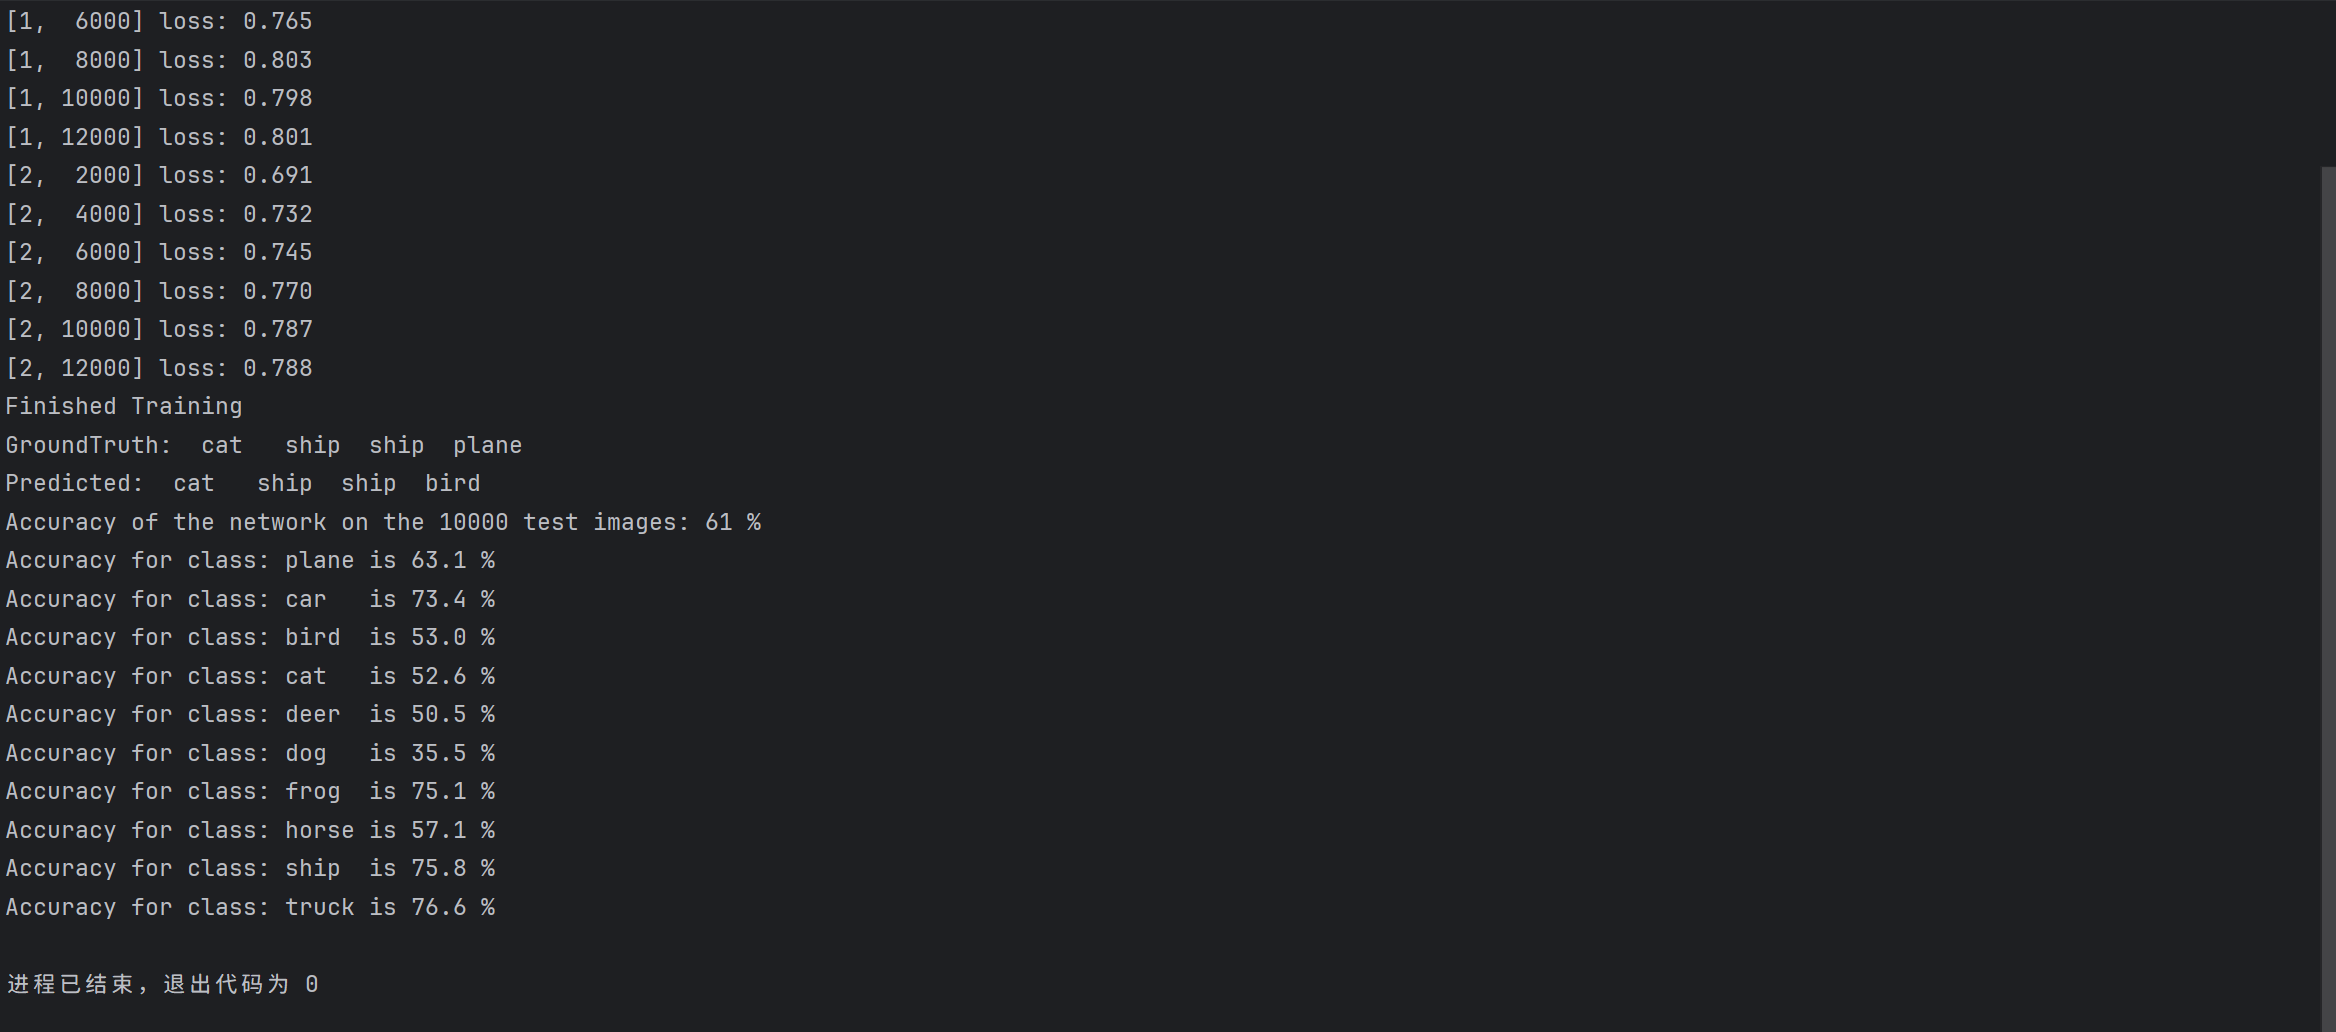
\includegraphics[width=0.45\linewidth]{PyTorch_3.png}
    }
    \caption{训练模型}
    \label{PyTorch}
\end{figure}

可以看到识别准确率还是比较堪忧,训练的效果还是不太好。

\end{document}